\documentclass[17pt,a4paper,landscape]{extarticle}
\usepackage[margin=2.35cm,top=0.12cm,left=1.05cm]{geometry}
\usepackage{amsmath}
\usepackage{amssymb}
\usepackage{tasks}
\usepackage{tikz}
\usepackage{xcolor}
\usepackage[sfdefault,lf]{FiraSans}
\renewcommand{\familydefault}{\sfdefault}
\setlength{\parindent}{0pt}
\pagestyle{empty}
\settasks{label=\textbf{\arabic*.}, label-width=2.2em, item-indent=2.95em, column-sep=2.1cm, after-item-skip=5.1em}
\renewcommand{\arraystretch}{1.15}
\everymath{\displaystyle}

\newcommand{\twocointree}{%
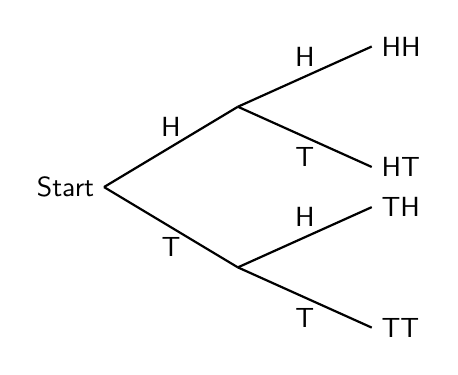
\begin{tikzpicture}[x=0.85cm,y=0.85cm]
  \draw[thick] (0,0) -- (2,1.2) node[midway,above] {H};
  \draw[thick] (0,0) -- (2,-1.2) node[midway,below] {T};
  \draw[thick] (2,1.2) -- (4,2.1) node[midway,above] {H};
  \draw[thick] (2,1.2) -- (4,0.3) node[midway,below] {T};
  \draw[thick] (2,-1.2) -- (4,-0.3) node[midway,above] {H};
  \draw[thick] (2,-1.2) -- (4,-2.1) node[midway,below] {T};
  \node[left] at (0,0) {Start};
  \node[right] at (4,2.1) {HH};
  \node[right] at (4,0.3) {HT};
  \node[right] at (4,-0.3) {TH};
  \node[right] at (4,-2.1) {TT};
\end{tikzpicture}%
}

\newcommand{\threetwothreetree}{%
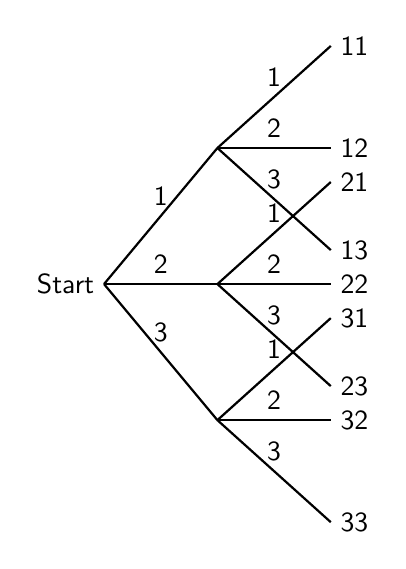
\begin{tikzpicture}[x=0.72cm,y=0.72cm]
  \foreach \y/\n in {2.4/1,0/2,-2.4/3} {
    \draw[thick] (0,0) -- (2,\y) node[midway,above] {\n};
  }
  \foreach \sy/\ey/\n/\lab in {2.4/4.2/1/11,2.4/2.4/2/12,2.4/0.6/3/13,0/1.8/1/21,0/0/2/22,0/-1.8/3/23,-2.4/-0.6/1/31,-2.4/-2.4/2/32,-2.4/-4.2/3/33} {
    \draw[thick] (2,\sy) -- (4,\ey) node[midway,above] {\n};
    \node[right] at (4,\ey) {\lab};
  }
  \node[left] at (0,0) {Start};
\end{tikzpicture}%
}


\begin{document}
\sffamily
\boldmath

\vspace*{0.4em}
{\LARGE \textbf{Proficient}}
\begin{tasks}(2)
\task {Use this tree to list the full sample space for two fair coin tosses.

\vspace{0.4em}\twocointree}
\task {Use the tree to find the probability of getting exactly two heads.

\vspace{0.4em}\twocointree}
\task {Use the tree to find the probability of getting at least one head.

\vspace{0.4em}\twocointree}
\task {Use this tree for a spinner labelled $1,2,3$ spun twice. List the outcomes where the total is $4$.

\vspace{0.4em}\threetwothreetree}
\task {Use the tree to find the probability that the total is $4$.

\vspace{0.4em}\threetwothreetree}
\task {A fair die is rolled twice. What is the probability of getting a $6$ then an even number?}
\task {A fair die is rolled twice. What is the probability that both numbers are odd?}
\task {A bag has $2$ red and $1$ blue counter. A counter is picked, replaced, then picked again. What is the probability of red then blue?}
\task {A bag has $2$ red and $1$ blue counter. A counter is picked, replaced, then picked again. What is the probability of two blues?}
\task {A fair coin is tossed twice. What is the probability of getting the same result both times?}
\task {A fair coin is tossed twice. What is the probability of getting different results?}
\task {Fill in the blank: for two fair coin tosses, the probability of exactly one head is $\frac{\square}{4}$.}
\task {Fill in the blank: for two fair die rolls, the probability of getting two odd numbers is $\frac{\square}{36}$.}
\task {Which is greater: the probability of two heads in two coin tosses or the probability of a $6$ then a $6$ in two die rolls?}
\task {Which is smaller: the probability of red then blue from a red-blue spinner spun twice or the probability of two reds?}
\task {A student says the probability of H then $5$ when a coin is tossed and a die is rolled is $\frac{1}{6}$. Are they correct?}
\task {Explain in one short sentence what a branch on a tree diagram shows.}
\end{tasks}

\end{document}
